%%%%%%%%%%%%%%%%%%%%%%%%%%%%%%%%%%%%%%%%%%%%%%%%%%%%%%%%%%%%%%%%%%%%%%%%%%%%%%%%%%%%%
%%%%%%%%%%%%%%%%%%%%%%%%%%%%%%%%%%%%%%%%%%%%%%%%%%%%%%%%%%%%%%%%%%%%%%%%%%%%%%%%%%%%%

\setbeamercolor{block title}{bg=white, fg=black}
\setbeamercolor{body}{bg=blue!20}

%%%%%%%%%%%%%%%%%%%%%%%%%%%%%%%%%%%%%%%%%%%%%%%%%%%%%%%%%%%%%%%%%%%%%%%%%%%%%%%%%%%%%%
%%%%%%%%%%%%%%%%%%%%%%%%%%%%%%%%%%%%%%%%%%%%%%%%%%%%%%%%%%%%%%%%%%%%%%%%%%%%%%%%%%%%%%

\begin{frame}
	\frametitle{Problem}
	\begin{itemize}
		\item All compilers contains bugs
		\item Relatively new programming language Kotlin compiler --- not an exclusion
	\end{itemize}
\end{frame}


%%%%%%%%%%%%%%%%%%%%%%%%%%%%%%%%%%%%%%%%%%%%%%%%%%%%%%%%%%%%%%%%%%%%%%%%%%%%%%%%%%%%%%
%%%%%%%%%%%%%%%%%%%%%%%%%%%%%%%%%%%%%%%%%%%%%%%%%%%%%%%%%%%%%%%%%%%%%%%%%%%%%%%%%%%%%%

\begin{frame}
	\frametitle{Main problem in compiler fuzzing}
\setbeamercolor{postit}{bg=red!20}
	\begin{beamercolorbox}[sep=1em]{postit}
		\centering
		How to generate random, non-trivial and semantically valid program to test the compiler?
	\end{beamercolorbox}

\end{frame}


%%%%%%%%%%%%%%%%%%%%%%%%%%%%%%%%%%%%%%%%%%%%%%%%%%%%%%%%%%%%%%%%%%%%%%%%%%%%%%%%%%%%%%
%%%%%%%%%%%%%%%%%%%%%%%%%%%%%%%%%%%%%%%%%%%%%%%%%%%%%%%%%%%%%%%%%%%%%%%%%%%%%%%%%%%%%%

\begin{frame}
	\frametitle{Existing methods}
	\begin{itemize}
		\item Grammar-aware generation ``CSmith'' approaches
			\begin{itemize}
				\item CSmith
				\item YARPGen
				\item jsfunfuzz
				\item ...
			\end{itemize}
	\end{itemize}
\end{frame}

%%%%%%%%%%%%%%%%%%%%%%%%%%%%%%%%%%%%%%%%%%%%%%%%%%%%%%%%%%%%%%%%%%%%%%%%%%%%%%%%%%%%%%
%%%%%%%%%%%%%%%%%%%%%%%%%%%%%%%%%%%%%%%%%%%%%%%%%%%%%%%%%%%%%%%%%%%%%%%%%%%%%%%%%%%%%%

\begin{frame}
	\frametitle{Existing methods}
	\begin{itemize}
		\item Mutation approaches
			\begin{itemize}
				\item jsfunfuzz
				\item ...
				\item skeletal program enumeration
			\end{itemize}
	\end{itemize}
	
\end{frame}

%%%%%%%%%%%%%%%%%%%%%%%%%%%%%%%%%%%%%%%%%%%%%%%%%%%%%%%%%%%%%%%%%%%%%%%%%%%%%%%%%%%%%%
%%%%%%%%%%%%%%%%%%%%%%%%%%%%%%%%%%%%%%%%%%%%%%%%%%%%%%%%%%%%%%%%%%%%%%%%%%%%%%%%%%%%%%

\begin{frame}[fragile]
	\frametitle{Skeletal program enumeration}
\begin{minipage}{0.4\linewidth}
Program P:
		\begin{lstlisting}[language=Kotlin]
var a: Int = 1
var b: Int = 1

while (b < 100) {
    val c = b
    b = a + b
    a = c
}
 \end{lstlisting}
	\end{minipage}
	\begin{minipage}{0.1\linewidth}
	\ \ 
	\end{minipage}
	\begin{minipage}{0.4\linewidth}
Skeleton P':
		\begin{lstlisting}[language=Kotlin]
var [_]: Int = 1
var [_]: Int = 1

while ([_] < 100) {
    val [_] = [_]
    [_] = [_] + [_]
    [_] = [_]
}
	\end{lstlisting}
\end{minipage}
	
\end{frame}


%%%%%%%%%%%%%%%%%%%%%%%%%%%%%%%%%%%%%%%%%%%%%%%%%%%%%%%%%%%%%%%%%%%%%%%%%%%%%%%%%%%%%%
%%%%%%%%%%%%%%%%%%%%%%%%%%%%%%%%%%%%%%%%%%%%%%%%%%%%%%%%%%%%%%%%%%%%%%%%%%%%%%%%%%%%%%

\begin{frame}[fragile]
	\frametitle{Skeletal program enumeration}
\begin{minipage}{0.4\linewidth}
Skeleton P':
		\begin{lstlisting}[language=Kotlin]
var [_]: Int = 1
var [_]: Int = 1

while ([_] < 100) {
    val [_] = [_]
    [_] = [_] + [_]
    [_] = [_]
}
 \end{lstlisting}
	\end{minipage}
	\begin{minipage}{0.1\linewidth}
	\ \ 
	\end{minipage}
	\begin{minipage}{0.4\linewidth}
Produced program P1:
		\begin{lstlisting}[language=Kotlin]
var a: Int = 1
var c: Int = 1

while (a < 100) {
    val b = a
    c = a + c
    a = c
}
	\end{lstlisting}
\end{minipage}
	
\setbeamercolor{postit}{bg=green!20}
	\begin{beamercolorbox}[sep=1em]{postit}
		\centering
		200+ GCC/Clang bugs
	\end{beamercolorbox}
\end{frame}

%%%%%%%%%%%%%%%%%%%%%%%%%%%%%%%%%%%%%%%%%%%%%%%%%%%%%%%%%%%%%%%%%%%%%%%%%%%%%%%%%%%%%%
%%%%%%%%%%%%%%%%%%%%%%%%%%%%%%%%%%%%%%%%%%%%%%%%%%%%%%%%%%%%%%%%%%%%%%%%%%%%%%%%%%%%%%


\begin{frame}[fragile]
	\frametitle{Type-centric fuzzing}
	\begin{itemize}
		\item Inspired by skeletal program enumeration
		\item Placeholders --- expressions
		\item Fill placeholders by compatible typed generated expressions
	\end{itemize}
\ \\ \ \\
\begin{minipage}{0.4\linewidth}
SPE:
\begin{lstlisting}[language=Kotlin]
val a: Int = 1
\end{lstlisting}
 \ \ \ \ \ \ \ \ \ \ \ \ $\downarrow$
\begin{lstlisting}[language=Kotlin]
val [_]: Int = 1
\end{lstlisting}
	\end{minipage}
	\begin{minipage}{0.1\linewidth}
	\ \ 
	\end{minipage}
	\begin{minipage}{0.4\linewidth}
TCE:
\begin{lstlisting}[language=Kotlin]
val a: Int = 1
\end{lstlisting}
 \ \ \ \ \ \ \ \ \ \ \ \ \ \ \ $\downarrow$
\begin{lstlisting}[language=Kotlin]
val a: Int = [Int]
\end{lstlisting}
\end{minipage}
\end{frame}

%%%%%%%%%%%%%%%%%%%%%%%%%%%%%%%%%%%%%%%%%%%%%%%%%%%%%%%%%%%%%%%%%%%%%%%%%%%%%%%%%%%%%%
%%%%%%%%%%%%%%%%%%%%%%%%%%%%%%%%%%%%%%%%%%%%%%%%%%%%%%%%%%%%%%%%%%%%%%%%%%%%%%%%%%%%%%

\begin{frame}[fragile]
	\frametitle{Type centric fuzzing example}
\begin{minipage}{0.4\linewidth}
Program P:
		\begin{lstlisting}[language=Kotlin,basicstyle=\footnotesize]
class A(val a: Int)

fun f(): Int {
    ...
}

var a: Int = 1
var b: Int = 1

while (b < 100) {
    val c = b
    b = a + b
    a = c
}
 \end{lstlisting}
	\end{minipage}
	\begin{minipage}{0.1\linewidth}
	\ \ 
	\end{minipage}
	\begin{minipage}{0.4\linewidth}
Skeleton P':
		\begin{lstlisting}[language=Kotlin,basicstyle=\footnotesize]
class A(val a: Int)

fun f(): Int {
    ...
}

var a: Int = [Int]
var b: Int = [Int]

while ([Int] < [Int]) {
    val c = [Int]
    [Int] = [[Int] + [Int]]
    [Int] = [Int]
}
	\end{lstlisting}
\end{minipage}
	
\end{frame}

%%%%%%%%%%%%%%%%%%%%%%%%%%%%%%%%%%%%%%%%%%%%%%%%%%%%%%%%%%%%%%%%%%%%%%%%%%%%%%%%%%%%%%
%%%%%%%%%%%%%%%%%%%%%%%%%%%%%%%%%%%%%%%%%%%%%%%%%%%%%%%%%%%%%%%%%%%%%%%%%%%%%%%%%%%%%%

\begin{frame}[fragile]
	\frametitle{Type centric fuzzing example}
\begin{minipage}{0.4\linewidth}
Skeleton P':
		\begin{lstlisting}[language=Kotlin,basicstyle=\footnotesize]
class A(val a: Int)

fun f(): Int {
    ...
}

var a: Int = [Int]
var b: Int = [Int]

while ([Int] < [Int]) {
    val c = [Int]
    [Int] = [[Int] + [Int]]
    [Int] = [Int]
}
 \end{lstlisting}
	\end{minipage}
	\begin{minipage}{0.1\linewidth}
	\ \ 
	\end{minipage}
	\begin{minipage}{0.4\linewidth}
Produced program P1:
		\begin{lstlisting}[language=Kotlin,basicstyle=\footnotesize]
class A(val a: Int)

fun f(): Int {
    ...
}

var a: Int = -100
var b: Int = a * f()

while (a < b) {
    val c = 12345
    b = A(f()).a
    b = b
}
	\end{lstlisting}
\end{minipage}
	
\end{frame}

%%%%%%%%%%%%%%%%%%%%%%%%%%%%%%%%%%%%%%%%%%%%%%%%%%%%%%%%%%%%%%%%%%%%%%%%%%%%%%%%%%%%%%
%%%%%%%%%%%%%%%%%%%%%%%%%%%%%%%%%%%%%%%%%%%%%%%%%%%%%%%%%%%%%%%%%%%%%%%%%%%%%%%%%%%%%%

\begin{frame}
	\frametitle{Type-centric fuzzing scheme}
		\begin{itemize}
			\item Generate expressions to fill the placeholders (generation phase)
			\item Fill skeleton by generated expressions (mutation phase)
		\end{itemize}
\end{frame}
%%%%%%%%%%%%%%%%%%%%%%%%%%%%%%%%%%%%%%%%%%%%%%%%%%%%%%%%%%%%%%%%%%%%%%%%%%%%%%%%%%%%%%
%%%%%%%%%%%%%%%%%%%%%%%%%%%%%%%%%%%%%%%%%%%%%%%%%%%%%%%%%%%%%%%%%%%%%%%%%%%%%%%%%%%%%%

\begin{frame}[fragile]
	\frametitle{Generation phase}
	Given:
	\begin{itemize}
		\item Set of variables $V$ 
		\item Available callables $C$
	\end{itemize}
	\ \\ \ \\
			\begin{lstlisting}[language=Kotlin,basicstyle=\footnotesize]
class A(                             //c1
    val a: Int                       //c2
) {                
    fun f(a: String): Int { ... }    //c3
}

val a: Int = 1                       //v1

		\end{lstlisting}
\end{frame}

%%%%%%%%%%%%%%%%%%%%%%%%%%%%%%%%%%%%%%%%%%%%%%%%%%%%%%%%%%%%%%%%%%%%%%%%%%%%%%%%%%%%%%
%%%%%%%%%%%%%%%%%%%%%%%%%%%%%%%%%%%%%%%%%%%%%%%%%%%%%%%%%%%%%%%%%%%%%%%%%%%%%%%%%%%%%%

\begin{frame}[fragile]
	\frametitle{Generation phase}
	We need to generate set of typed expressions using the $C$:
\begin{lstlisting}[language=Kotlin,basicstyle=\footnotesize]
class A(                             //A(1) -> A
    val a: Int                       //A(1).a -> Int
) {                
    fun f(a: String): Int { ... }    //A(1).f("") -> Int
}
\end{lstlisting}
\end{frame}

%%%%%%%%%%%%%%%%%%%%%%%%%%%%%%%%%%%%%%%%%%%%%%%%%%%%%%%%%%%%%%%%%%%%%%%%%%%%%%%%%%%%%%
%%%%%%%%%%%%%%%%%%%%%%%%%%%%%%%%%%%%%%%%%%%%%%%%%%%%%%%%%%%%%%%%%%%%%%%%%%%%%%%%%%%%%%

\begin{frame}[fragile]
\frametitle{Generation phase algorithm}
\newcommand{\adaptTypeParameters}{\text{adaptTypeParams}}%
\newcommand{\args}{\mathit{args}}%
\newcommand{\callee}{\mathit{callee}}%
\newcommand{\call}{\mathit{call}}%
\newcommand{\ffile}{\mathit{file}}%
\newcommand{\findImplementation}{\text{findImplementation}}%
\newcommand{\generateCall}{\text{genCall}}%
\newcommand{\generateClassInstance}{\text{genClassInstance}}%
\newcommand{\generateConstructorCall}{\text{genConstructorCall}}%
\newcommand{\generateConstructor}{\text{genConstructor}}%
\newcommand{\generateInstance}{\text{genInstance}}%
\newcommand{\generateTypeParams}{\text{genTypeParams}}%
\newcommand{\generateValue}{\text{genValue}}%
\newcommand{\getCallables}{\text{getCallables}}%
\newcommand{\getInstanceCallables}{\text{getInstanceCallables}}%
\newcommand{\getRandomConstructor}{\text{getRandomConstructor}}%
\newcommand{\hasOpenConstructor}{\text{hasOpenConstructor}}%
\newcommand{\iCallee}{\mathit{iCallee}}%
\newcommand{\impl}{\mathit{impl}}%
\newcommand{\instance}{\mathit{instance}}%
\newcommand{\is}{\ \mathit{is}\ }%
\newcommand{\klass}{\mathit{class}}%
\newcommand{\parameterize}{\text{parameterize}}%
\newcommand{\randomCtor}{\mathit{randomCtor}}%
\newcommand{\res}{\mathit{res}}%
\newcommand{\typeParams}{\mathit{typeParams}}%
\newcommand{\usages}{\mathit{usages}}%


%%%%%%%%%%%%%%%%%%%%%%%%%%%%%%%%%%%%%%%%%%%%%%%%%%%%%%%%%%%%%%%%%%%%%%%%%%%%%%%
\algdef{SE}[FUNCTION]{Function}{EndFunction}%
   [2]{\algorithmicfunction\ \textproc{#1}\ifthenelse{\equal{#2}{}}{}{(#2)}}%
   {\algorithmicend\ \algorithmicfunction }

\begin{figure}[tb]
\setlength{\leftskip}{0cm}
\small
\textbf{INPUT:} $\ffile$ with a seed program $P$ \\
\textbf{OUTPUT:} list of generated expressions $c_0...c_N$ \\
\begin{algorithmic}[1]


\Function{generationPhase}{$\ffile$}
    \State $\res \leftarrow \left[ \, \right]$
    
    \For{$\callee \in \getCallables(\ffile)$}
        \If{$\callee \is Class$}
            \State $\instance \leftarrow \generateClassInstance(\callee, \ffile)$
            \For{$\iCallee \in \getCallables(\instance)$}
                \State $\res \leftarrow \res + \generateCall(\iCallee, \ffile)$
            \EndFor
        \Else
            \State $\res \leftarrow \res + \generateCall(\callee, \ffile)$
        \EndIf
    \EndFor
    \State \Return $\res$
\EndFunction

%\\
%\Function{genClassInstance}{$\klass, \ffile$}
%    \State $\typeParams \leftarrow \generateTypeParams(\klass, \ffile)$
%    \State $\klass \leftarrow \parameterize(\klass, \typeParams)$
%    \If{$ \neg \hasOpenConstructor(\klass)$}
%        \State $\impl \leftarrow \findImplementation(\klass)$
%        \If{$ \impl \neq null $}
%            \State $\impl \leftarrow \adaptTypeParameters($
%            \State $\qquad \impl, \klass, \typeParams)$
%            \State \Return $\generateClassInstance(\impl, \ffile)$
%        \Else
%            \State \Return $null$
%        \EndIf
%    \EndIf
%    \State $\randomCtor \leftarrow \getRandomConstructor(\klass)$
%    \State \Return $\generateConstructorCall(\randomCtor, \ffile)$
%\EndFunction

% \State $\args \leftarrow \left[ \, \right]$
% \For{$\arg \in \getArgs(\randomCtor)$}
%     \State $\args \leftarrow \args + \generateValue(\arg)$
% \EndFor

\end{algorithmic}
\end{figure}
\end{frame}

\begin{frame}[fragile]
\frametitle{Class instances generation algorithm}
\newcommand{\adaptTypeParameters}{\text{adaptTypeParams}}%
\newcommand{\args}{\mathit{args}}%
\newcommand{\callee}{\mathit{callee}}%
\newcommand{\call}{\mathit{call}}%
\newcommand{\ffile}{\mathit{file}}%
\newcommand{\findImplementation}{\text{findImplementation}}%
\newcommand{\generateCall}{\text{genCall}}%
\newcommand{\generateClassInstance}{\text{genClassInstance}}%
\newcommand{\generateConstructorCall}{\text{genConstructorCall}}%
\newcommand{\generateConstructor}{\text{genConstructor}}%
\newcommand{\generateInstance}{\text{genInstance}}%
\newcommand{\generateTypeParams}{\text{genTypeParams}}%
\newcommand{\generateValue}{\text{genValue}}%
\newcommand{\getCallables}{\text{getCallables}}%
\newcommand{\getInstanceCallables}{\text{getInstanceCallables}}%
\newcommand{\getRandomConstructor}{\text{getRandomConstructor}}%
\newcommand{\hasOpenConstructor}{\text{hasOpenConstructor}}%
\newcommand{\iCallee}{\mathit{iCallee}}%
\newcommand{\impl}{\mathit{impl}}%
\newcommand{\instance}{\mathit{instance}}%
\newcommand{\is}{\ \mathit{is}\ }%
\newcommand{\klass}{\mathit{class}}%
\newcommand{\parameterize}{\text{parameterize}}%
\newcommand{\randomCtor}{\mathit{randomCtor}}%
\newcommand{\res}{\mathit{res}}%
\newcommand{\typeParams}{\mathit{typeParams}}%
\newcommand{\usages}{\mathit{usages}}%


%%%%%%%%%%%%%%%%%%%%%%%%%%%%%%%%%%%%%%%%%%%%%%%%%%%%%%%%%%%%%%%%%%%%%%%%%%%%%%%
\algdef{SE}[FUNCTION]{Function}{EndFunction}%
   [2]{\algorithmicfunction\ \textproc{#1}\ifthenelse{\equal{#2}{}}{}{(#2)}}%
   {\algorithmicend\ \algorithmicfunction }

\begin{figure}[tb]
\setlength{\leftskip}{0cm}
\small

\begin{algorithmic}[1]
\Function{genClassInstance}{$\klass, \ffile$}
    \State $\typeParams \leftarrow \generateTypeParams(\klass, \ffile)$
    \State $\klass \leftarrow \parameterize(\klass, \typeParams)$
    \If{$ \neg \hasOpenConstructor(\klass)$}
        \State $\impl \leftarrow \findImplementation(\klass)$
        \If{$ \impl \neq null $}
            \State $\impl \leftarrow \adaptTypeParameters(\impl, \klass, \typeParams)$
            \State \Return $\generateClassInstance(\impl, \ffile)$
        \Else
            \State \Return $null$
        \EndIf
    \EndIf
    \State $\randomCtor \leftarrow \getRandomConstructor(\klass)$
    \State \Return $\generateConstructorCall(\randomCtor, \ffile)$
\EndFunction

\end{algorithmic}
\end{figure}
\end{frame}


%%%%%%%%%%%%%%%%%%%%%%%%%%%%%%%%%%%%%%%%%%%%%%%%%%%%%%%%%%%%%%%%%%%%%%%%%%%%%%%%%%%%%%
%%%%%%%%%%%%%%%%%%%%%%%%%%%%%%%%%%%%%%%%%%%%%%%%%%%%%%%%%%%%%%%%%%%%%%%%%%%%%%%%%%%%%%

\begin{frame}[fragile]
	\frametitle{Mutation phase}
	Given: 
		\begin{itemize}
			\item Set of generated on previous step expressions $E$
			\item Seed program for mutation phase
		\end{itemize}
	\ \\ \ \\
	\begin{lstlisting}[
  language=Kotlin, basicstyle=\footnotesize
]
// A(1) -> A           | e1
// A(1).a -> Int       | e2
// A(1).f("") -> Int   | e3
// a -> Int            | e4

fun factorial(n: Int): Double {
    var result = 1.0
    for (i in 1..n) {
        result *= i
    }
    return result
}
\end{lstlisting}
\end{frame}

%%%%%%%%%%%%%%%%%%%%%%%%%%%%%%%%%%%%%%%%%%%%%%%%%%%%%%%%%%%%%%%%%%%%%%%%%%%%%%%%%%%%%%
%%%%%%%%%%%%%%%%%%%%%%%%%%%%%%%%%%%%%%%%%%%%%%%%%%%%%%%%%%%%%%%%%%%%%%%%%%%%%%%%%%%%%%

\begin{frame}[fragile]
	\frametitle{Mutation phase}
	Need to make type placeholders and fill it by $e \in E$
	\\ \ \\ \ 
\begin{lstlisting}[
  language=Kotlin, basicstyle=\footnotesize
]
fun factorial(n: Int): Double {
    var result = [Double]
    for (i in [IntRange]) {
        [Double] *= [Int]
    }
    return [Double]
}
\end{lstlisting}
\end{frame}

%%%%%%%%%%%%%%%%%%%%%%%%%%%%%%%%%%%%%%%%%%%%%%%%%%%%%%%%%%%%%%%%%%%%%%%%%%%%%%%%%%%%%%
%%%%%%%%%%%%%%%%%%%%%%%%%%%%%%%%%%%%%%%%%%%%%%%%%%%%%%%%%%%%%%%%%%%%%%%%%%%%%%%%%%%%%%

\begin{frame}[fragile]
	\frametitle{Mutation phase example}
\begin{lstlisting}[
  language=Kotlin, basicstyle=\footnotesize
]
val a: Int = 1

class A(val a: Int) {
    fun f(a: String): Int { ... }
}

fun f(a: Int): Int { ... }

fun factorial(n: Int): Double {
    var result = f(1).toDouble()
    for (i in A(1).f("")..a) {
        result *= i
    }
    return result
}
\end{lstlisting}
\end{frame}

%%%%%%%%%%%%%%%%%%%%%%%%%%%%%%%%%%%%%%%%%%%%%%%%%%%%%%%%%%%%%%%%%%%%%%%%%%%%%%%%%%%%%%
%%%%%%%%%%%%%%%%%%%%%%%%%%%%%%%%%%%%%%%%%%%%%%%%%%%%%%%%%%%%%%%%%%%%%%%%%%%%%%%%%%%%%%

\begin{frame}[fragile]
	\frametitle{How to choose expression to fill?}
	\begin{itemize}
		\item Select a type-compatible expression from $E$
		\item Create a random value of a built-in type~(int, bool, etc.)
		\item Generate a valid call to the standard library
	\end{itemize}
\end{frame}

%%%%%%%%%%%%%%%%%%%%%%%%%%%%%%%%%%%%%%%%%%%%%%%%%%%%%%%%%%%%%%%%%%%%%%%%%%%%%%%%%%%%%%
%%%%%%%%%%%%%%%%%%%%%%%%%%%%%%%%%%%%%%%%%%%%%%%%%%%%%%%%%%%%%%%%%%%%%%%%%%%%%%%%%%%%%%

\begin{frame}[fragile]
	\frametitle{Generation of calls to the standard library}

\begin{lstlisting}[
  language=Kotlin, basicstyle=\footnotesize
]
                // a -> Int  |  [Double] 
\end{lstlisting}
\begin{lstlisting}[
  language=Kotlin, basicstyle=\tiny
]
n = 1:
fun and(other: Int): Int
fun dec(): Int
...
fun toDouble(): Double 
fun minus(other: Double): Double

n = 2:
fun toByte(): Byte
fun times(other: Double): Double

n = 3:
fun toFloat(): Byte
fun compareTo(other: Int): Int
fun plus(other: Double): Double

...

Generated:
a.toDouble()
a.minus(0.0)
a.toByte().times(2.2)
a.toFloat().compareTo(1).plus(0.0)
\end{lstlisting}

\end{frame}

%%%%%%%%%%%%%%%%%%%%%%%%%%%%%%%%%%%%%%%%%%%%%%%%%%%%%%%%%%%%%%%%%%%%%%%%%%%%%%%%%%%%%%
%%%%%%%%%%%%%%%%%%%%%%%%%%%%%%%%%%%%%%%%%%%%%%%%%%%%%%%%%%%%%%%%%%%%%%%%%%%%%%%%%%%%%%

\newcommand{\anon}{\mathit{anon}}%
\newcommand{\anonymize}{\text{anonymize}}%
\newcommand{\eType}{\mathit{eType}}%
\newcommand{\gen}{\mathit{gen}}%
\newcommand{\genPhExpr}{\text{genPhExpr}}%
\newcommand{\genRandomValue}{\text{genRandomValue}}%
\newcommand{\genStdLib}{\text{genStdLib}}%
\newcommand{\getPlaceholders}{\text{getPlaceholders}}%
\newcommand{\getType}{\text{getType}}%
\newcommand{\merge}{\text{merge}}%
\newcommand{\replacePhWithExpr}{\text{replacePhWithExpr}}%
\newcommand{\seed}{\mathit{seed}}%
\newcommand{\type}{\mathit{type}}%

\begin{frame}[fragile]
	\frametitle{Mutation phase algorithm}
\begin{figure}[tb]
\setlength{\leftskip}{0cm}
\textbf{INPUT:} seed program from generation phase $\gen$ \\
\textbf{INPUT:} generated expressions $exprs$ \\
\textbf{INPUT:} seed program for mutation phase $\seed$ \\
\textbf{OUTPUT:} program will filled type placeholders \\
\begin{algorithmic}[1]

\Function{mutationPhase}{}
    \State $\anon \leftarrow \anonymize(\seed)$
    \State $\anon \leftarrow \merge(\anon, \gen)$
    \For{$ph \in \getPlaceholders(\anon)$}
        \State $e \leftarrow \genPhExpr(ph, exprs)$
        \State $\anon \leftarrow \replacePhWithExpr(anon, ph, e)$
    \EndFor
    \State \Return{$\anon$}
\EndFunction
\end{algorithmic}
\end{figure}
\end{frame}

\begin{frame}[fragile]
	\frametitle{Generate phi expression algorithm}
\begin{figure}[tb]
\setlength{\leftskip}{0cm}
\begin{algorithmic}[1]

\Function{genPhExpr}{$ph, exprs$}
    \State $\type \leftarrow \getType(ph)$
    \State $r \leftarrow \left[ \, \right]$
    \State $r \leftarrow r + \genRandomValue(\type)$
    \State $r \leftarrow r + \genStdLib(\type)$
    \For{$e \in exprs$}
        \State $\eType \leftarrow \getType(ph)$
        \If{$compatible(\type, \eType)$}
            \State $r \leftarrow r + e$
        \EndIf
    \EndFor
    \State \Return{$random(r)$}
\EndFunction
\end{algorithmic}
\end{figure}
\end{frame}

%%%%%%%%%%%%%%%%%%%%%%%%%%%%%%%%%%%%%%%%%%%%%%%%%%%%%%%%%%%%%%%%%%%%%%%%%%%%%%%%%%%%%%
%%%%%%%%%%%%%%%%%%%%%%%%%%%%%%%%%%%%%%%%%%%%%%%%%%%%%%%%%%%%%%%%%%%%%%%%%%%%%%%%%%%%%%

\begin{frame}[fragile]
	\frametitle{Mutation phase?}
	Mutation phase can be applied many times:
\center{
\begin{lstlisting}[
  language=Kotlin
]
                    [List<Int>] 
\end{lstlisting}
$\downarrow$
\begin{lstlisting}[
  language=Kotlin
]
                  listOf(1, 2, 3)
\end{lstlisting}
$\downarrow$
\begin{lstlisting}[
  language=Kotlin
]
             listOf([Int], [Int], [Int])
\end{lstlisting}
}
\end{frame}
%%%%%%%%%%%%%%%%%%%%%%%%%%%%%%%%%%%%%%%%%%%%%%%%%%%%%%%%%%%%%%%%%%%%%%%%%%%%%%%%%%%%%%
%%%%%%%%%%%%%%%%%%%%%%%%%%%%%%%%%%%%%%%%%%%%%%%%%%%%%%%%%%%%%%%%%%%%%%%%%%%%%%%%%%%%%%


\begin{frame}
	\frametitle{TCE problems}
	\begin{itemize}
		\item The generation process could potentially never terminate
		\item With iterative TCE run time could increase nonlinearly
		\item Long chains of callables
	\end{itemize}
\end{frame}

%%%%%%%%%%%%%%%%%%%%%%%%%%%%%%%%%%%%%%%%%%%%%%%%%%%%%%%%%%%%%%%%%%%%%%%%%%%%%%%%%%%%%%
%%%%%%%%%%%%%%%%%%%%%%%%%%%%%%%%%%%%%%%%%%%%%%%%%%%%%%%%%%%%%%%%%%%%%%%%%%%%%%%%%%%%%%

\begin{frame}
	\frametitle{Implementation}
We have implemented our approach inside a tool for Kotlin compiler fuzzing named Backend Bug Finder (BBF):
	\begin{figure}
		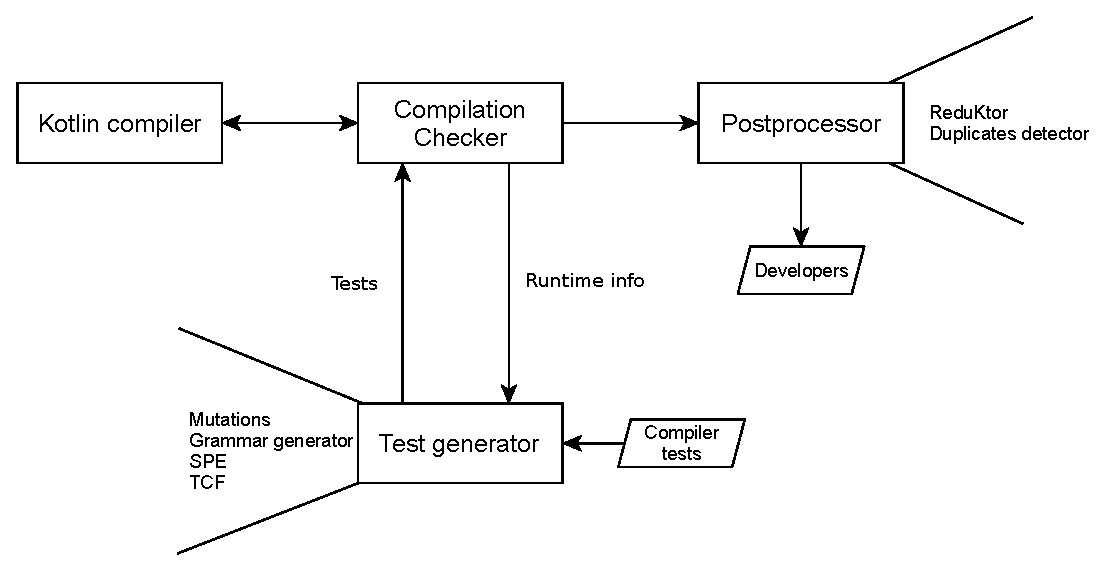
\includegraphics[width=100mm]{image/bbf_scheme}
	\end{figure}	
\end{frame}

%%%%%%%%%%%%%%%%%%%%%%%%%%%%%%%%%%%%%%%%%%%%%%%%%%%%%%%%%%%%%%%%%%%%%%%%%%%%%%%%%%%%%%

\begin{frame}[fragile]
	\frametitle{Evaluation}
	\begin{itemize}
		\item After running TCF for 2 weeks we found more than 50 unique, previously not reported bugs
		\item We deduplicated them and filtered ``uninteresting''
	\end{itemize}
	\begin{minipage}{0.4\linewidth}
Interesting bug:
		\begin{lstlisting}[language=Kotlin,basicstyle=\tiny]
fun box() {
    when ("abcd".sumOf { 1L }) {
        in 0..1 -> "A"
        else -> "B"
    }
}
 \end{lstlisting}
	\end{minipage}
	\begin{minipage}{0.1\linewidth}
	\ \ 
	\end{minipage}
	\begin{minipage}{0.4\linewidth}
Uninteresting bug:
		\begin{lstlisting}[language=Kotlin,basicstyle=\tiny, escapechar = |]
		
fun box() = 
fun() = 
::intArrayOf
	|
	|
	|
	\end{lstlisting}
\end{minipage}
\end{frame}
%%%%%%%%%%%%%%%%%%%%%%%%%%%%%%%%%%%%%%%%%%%%%%%%%%%%%%%%%%%%%%%%%%%%%%%%%%%%%%%%%%%%%%

\begin{frame}[fragile]
	\frametitle{Evaluation}
	After 2 weeks of fuzzing:
	\ \\ \ \\ \ \\
\scalebox{0.85}{
\begin{tabular}{| c | c | c | c | c |}
\hline

\multirow{1}{*}{\bf } & \multicolumn{1}{c|}{\bf NO SEVERITY} & \multicolumn{1}{c|}{\bf MINOR} & \multicolumn{1}{c|}{\bf NORMAL} & \multicolumn{1}{c|}{\bf MAJOR} \\
\hline
Frontend
& 2 & 0 & 0 & 0  \\
\hline
Backend
& 0 & 1 & 5 & 4 \\
\hline
Miscompilation
& 0 & 0 & 2 & 4 \\
\hline
\end{tabular}
}
\end{frame}

%%%%%%%%%%%%%%%%%%%%%%%%%%%%%%%%%%%%%%%%%%%%%%%%%%%%%%%%%%%%%%%%%%%%%%%%%%%%%%%%%%%%%%

\begin{frame}[fragile]
	\frametitle{Comparison with another approaches}

\scalebox{0.85}{
\begin{tabular}{| c | r | r | r | r | r | r | r |}
\hline

\multirow{1}{*}{\bf Results} & \multicolumn{1}{c|}{\bf M} & \multicolumn{1}{c|}{\bf G} & \multicolumn{1}{c|}{\bf EM} & \multicolumn{1}{c|}{\bf SPE} & \multicolumn{1}{c|}{\bf TCE} & \multicolumn{1}{c|}{\bf TCE + EM }  \\
\hline
Correct programs, \%
& 11.9 & 0.05 & 10.7 & 24.2 & 63.4 & 13.4\\
\hline
Interesting bugs, \%
& 25.0 & 0.0 & 20.0 & 100.0 & 100.0 & 16.6\\
\hline
Frontend crashes
& 3 & 212 & 4 & 0 & 0 & 5\\
\hline
Backend crashes
& 9 & 0 & 11 & 2 & 3 & 7\\
\hline
Miscompilations
& 0 & 0 & 0 & 0 & 3 & 0\\
\hline
Duplicates
& 49 & 77 & 38 & 1 & 4 & 14\\
\hline
\end{tabular}
}

\footnotesize{
\begin{itemize}
    \item (M) Mutation-based fuzzing;
    \item (G) Grammar based generation;
    \item (EM) M + language-specific mutations;
    \item (SPE) Skeletal program enumeration;
    \item (TCE) Type-centric enumeration;
    \item (TCE + EM) TCE + language-specific mutations.
\end{itemize}
}

\end{frame}

%%%%%%%%%%%%%%%%%%%%%%%%%%%%%%%%%%%%%%%%%%%%%%%%%%%%%%%%%%%%%%%%%%%%%%%%%%%%%%%%%%%%%%

\begin{frame}[fragile]
	\frametitle{Cumulative number of interesting bugs found per day}
	\begin{figure}
\begin{tikzpicture}
\begin{axis}[
    x label style={at={(axis description cs:0.5,-0.1)},anchor=north},
    y label style={at={(axis description cs:.1,.5)},anchor=south},
    xlabel={\#days}, 
    ylabel={\#found bugs},
    ymin=0, ymax=20,
    minor y tick num = 4,
    minor x tick num = 1,
    area style,
    tick align=outside,
    ]
\addplot+[fill=black,ybar interval,mark=none,draw=black] 
plot coordinates { 
(0, 3) (1, 6) (2, 8) (3, 8) (4, 9) (5, 10) (6, 11) (7, 11)
(8, 12) (9, 14) (10, 14) (11, 15) (12, 16) (13, 18) (14, 0) 
};
\end{axis}
\end{tikzpicture}
\end{figure}
\end{frame}

%%%%%%%%%%%%%%%%%%%%%%%%%%%%%%%%%%%%%%%%%%%%%%%%%%%%%%%%%%%%%%%%%%%%%%%%%%%%%%%%%%%%%%

\begin{frame}[fragile]
	\frametitle{Interesting bugs found}
	IR backend crash~(KT-42092):
	\ \\ \ \\
\begin{lstlisting}[
  language=Kotlin
]
fun box() {
    val l = ArrayList<Long>()
    l.add(@[Int]@) -> l.add(~5.inv()~)
}
\end{lstlisting}

\end{frame}

%%%%%%%%%%%%%%%%%%%%%%%%%%%%%%%%%%%%%%%%%%%%%%%%%%%%%%%%%%%%%%%%%%%%%%%%%%%%%%%%%%%%%%
\begin{frame}[fragile]
	\frametitle{Interesting bugs found}
	Miscompilation in default backend (KT-42064):
	\ \\ \ \\
\begin{lstlisting}[
  language=Kotlin
]
class Kl1 : HashSet<String>()
open class Kl2(par0: Any, par1: Any)

fun box1() =
    object : Kl2(
        par1 = "",
        par0 = @[String]@ -> ~Kl1().iterator().next()~
    ) {}
\end{lstlisting}

\end{frame}

%%%%%%%%%%%%%%%%%%%%%%%%%%%%%%%%%%%%%%%%%%%%%%%%%%%%%%%%%%%%%%%%%%%%%%%%%%%%%%%%%%%%%%

\begin{frame}
	\frametitle{Discussion?}
	\begin{itemize}
		\item Generalizability of type-centric fuzzing
		\item Scalability of type-centric enumeration
		\item Seed selection
		\item Project-level fuzzing
	\end{itemize}
\end{frame}

%%%%%%%%%%%%%%%%%%%%%%%%%%%%%%%%%%%%%%%%%%%%%%%%%%%%%%%%%%%%%%%%%%%%%%%%%%%%%%%%%%%%%%
%%%%%%%%%%%%%%%%%%%%%%%%%%%%%%%%%%%%%%%%%%%%%%%%%%%%%%%%%%%%%%%%%%%%%%%%%%%%%%%%%%%%%%

\begin{frame}
	\frametitle{Conclusion}
	4 pictures?
\end{frame}

%%%%%%%%%%%%%%%%%%%%%%%%%%%%%%%%%%%%%%%%%%%%%%%%%%%%%%%%%%%%%%%%%%%%%%%%%%%%%%%%%%%%%%%

\begin{frame}[fragile]
\frametitle{Contact information}
\texttt{\{stepanov, akhin, belyaev\}@kspt.icc.spbstu.ru} \\ \ \\ \ \\
\begin{columns} 
\column{0.33\textwidth} 
	\begin{figure}
		\includegraphics[width=0.99\linewidth]{image/polytech_logo_en} 
	\end{figure}
\column{0.33\textwidth} 
	\begin{figure}
		\includegraphics[width=0.99\linewidth]{image/jetbrainsLogo} 
	\end{figure}
\end{columns}
	\begin{figure}
		\includegraphics[width=0.4\linewidth]{image/Reduktor} 
	\end{figure}
\end{frame}